\documentclass[journal,letterpaper]{article}

%Imports

\usepackage[utf8]{inputenc}
%headings
\usepackage{fancyhdr}
%double-space
\usepackage{setspace}
%\say command
\usepackage{dirtytalk}
%variable margins
\usepackage{geometry}
%make the margins a bit less ridiculous
\newgeometry{top=1in,bottom=1.5in,left=1in,right=1in}
%images
\usepackage{graphicx}
\pagestyle{fancy}

\usepackage{tikz}
\usetikzlibrary{arrows}


\title{Dream Design - Better Apple Watch}
\author{Edward Seim}


\begin{document}
    \maketitle
    
    \section{Introduction}
    \label{introduction}

    As an avid advocate of the Pebble Watch, the main thing that dissappoints me about the Apple Watch is the simplicity that is lost by bringing the complexity of iPhone apps to the watch screen. The root of this problem is the use of the touchscreen. As a Pebble user, which has only buttons to use the device with, it makes it possible to use the watch with minimal thought and once you've used it for a while, you can eve perform tasks without looking at it. My goal with my improved Apple Watch interface is to minimize use of the touchscreen to only when its eseential.

    \begin{figure}[htbp]
        \centering
        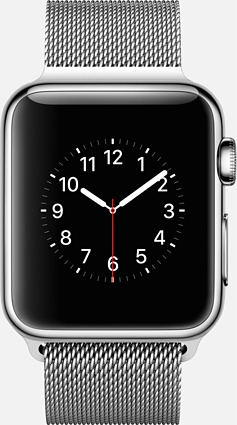
\includegraphics[width=10cm,height=10cm,keepaspectratio]{apple-watch}
        \caption{Apple Watch}
        \label{fig:apple_watch}
    \end{figure}

    \section{System}
    \label{System}

    Without any change to the hardware, the Apple Watch has the neccesary buttons to emulate a Pebble type simplicity. using the Digital crown as a select and scrolling mechanism, and the side button as the back button, you have the same capabilities as the Pebble Watch, with the advantage of the touchscreen for specific uses and the better screen to display better eye candy.

    The most important change to the overall design of the interface is the change over to a menu type system. This means that the root level is the watch face. Hitting the Digital Crown will go into the main menu. Scrolling on this top menu will show the various different apps that you want use, for example the messaging or music apps. Hitting the back button will take you up a level in the menus. As a general principle, when there is content on the screen and scrolling lets you see more content while hitting the crown gives you the actions that can be performed in that context with that content. The actions will be sorted by highest use case. For example, in a text notification, the highest case would be \say{dismiss}, while the next option would be \say{reply}.

    An important thing to note is that at any point, the digital crown can be held down to bring up Siri, which can act upon the current content or anything in the global context.

    \section{Examples}
    \label{examples}

    \subsection{Message Notification}

    Fully fleshing out the idea presented earlier, we are looking at the case of recieving a message notification.

    In its natural state, Apple Watch is showing the main watchface. A message comes in and overlays over the watchface and indicates to the user that a notification has come in by firing off the Taptic Engine. Whats on the screen is something resembling the current Apple Watch, as seen in Figure \ref{fig:messages}. The dot next immediately next to the digital crown represents that there are actions that can be performed on this content. Figure \ref{fig:messages_actions} represents some of the actions that can be done on a message notification. Note that the \say{dismiss} option is currently selected. 

    Within a message notifcation, the Siri context includes things like dismiss and reply, where you can immediately dictate a responce by saying something like \say{Reply \say{I'll be home soon}}.

    \begin{figure}[htbp]
        \centering
        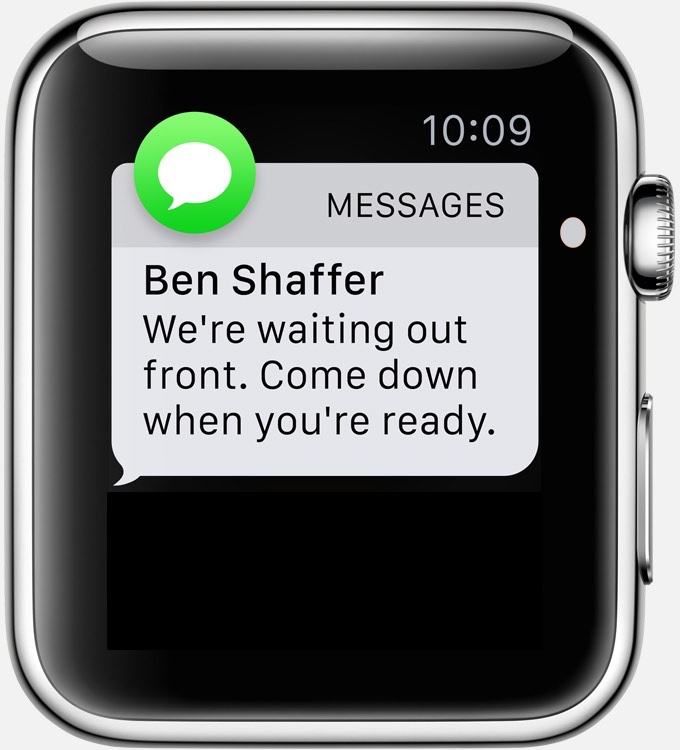
\includegraphics[width=10cm,height=8cm,keepaspectratio]{messages}
        \caption{Messages Main Content}
        \label{fig:messages}
    \end{figure}

    \begin{figure}[htbp]
        \centering
        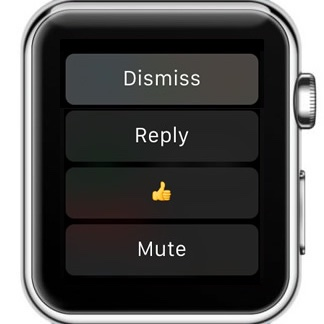
\includegraphics[width=10cm,height=8cm,keepaspectratio]{messages-actions}
        \caption{Messages Actions}
        \label{fig:messages_actions}
    \end{figure}

    \subsection{Music App}

    The Music app would be one of the apps listed in the top level menu directly beneath the watchface. You would see the song currently playing with corresponding artist and album names along with a playhead indicator and beautiful album artwork. Again, an indicator would be present next to the digital crown to indicate actions can be done on this content. The primary option would be to Play/Pause. Others would include volume and scrubbing, which would each present a vertical bar that can be manipulated with scrolling to get to the desired volume or playhead. Scrolling on the content, aka the currently playing song, would bring you to the full library. In this context, the actions that would be presented for this content would be different than that for the \say{Now Playing}. Things to change the view like sorting by artists, albums, or songs would be presented, along with the option for viewing playlsits.

    Within the Music App, the Siri context includes things like playing specific songs, artists, albums, playlists, along with changing the volume or playhead. For example, saying \say{Play songs by The Killers} would make Apple Watch start playback of songs by \say{The Killers} on the default listening interface. 

    \subsection{Yo App}
    
    Looking at a specific API, the Yo API seems the most applcable to a watch use because of its simplicity. This is something important to keep in mind with a watch application. Simplicity will mean you can get tasks done quickly and without much chance for user error.

    By opening the Yo app you have indicated that you wish to send a yo, as thats the only reason you would need to open the app. As such, the menu you are immediately presented with is the list of yo users you have configured already to send to. Simply scrolling to that user you wish to send a yo to and hitting the digital crown will prompt the sending of a yo to that user. The last option at the bottom of the list of users is an add button, which brings up Siri to dictate the user you wish to add.

    The Siri context within the Yo app includes performing actions like sending a yo to a specific user and adding a new user.

    \section{Conclusion}
    \label{conclusion}

    Nec cu eripuit nostrum, at pro reque velit graeci. Pri graeco iisque conceptam te. Ius dolore melius contentiones in, pro eius ponderum ei. Aperiri tamquam voluptua nec cu, eu pri quaeque constituto, eam ne sumo commune menandri. Duo iudico legimus cu, iudicabit scriptorem vis eu. Mel nonumy possit scaevola ex, ea idque blandit vel.

    An blandit accumsan qui, id vis erant inermis. Impedit facilis platonem duo et. Eum corpora blandit te, regione consequat dissentiunt per ut, labitur philosophia pro at. Nam saepe admodum antiopam at. Nam no meis malorum erroribus, duo ea doctus probatus expetendis.

    Eius commodo oporteat mea in, no vix labores denique. Cum ne alia quodsi. Ei sea lorem aliquam mediocrem, eu invidunt delicata mandamus eos, cu quis platonem mei. Timeam albucius assueverit id eum, mel ad nusquam insolens, impetus repudiare mel no. Cu mentitum adipisci tacimates vel, has populo reformidans in.

    Inimicus necessitatibus cum et, in ullum molestiae appellantur mei. Et zril scaevola consetetur sea. Eu sed natum fabulas assentior. Ex solum impetus repudiare mea, in veritus salutandi liberavisse quo. At sea quot iusto voluptatibus, maiorum concludaturque at eam, lorem dicat mea at.

    Legendos accusata antiopam et pro. Cum et atqui timeam appellantur, vis electram consetetur cu. Te nec neglegentur concludaturque, duo an admodum facilisis repudiare, est ea esse persecuti. Amet partiendo mnesarchum at eos, reque argumentum suscipiantur duo cu. Et sonet convenire assueverit vel, vide tollit id his, indoctum tractatos eum ne.

    Mel in probatus mandamus repudiare. Paulo evertitur mea ne, erroribus forensibus mel ut, ei mea nonumes graecis habemus. Id virtute inermis accusamus has, ius albucius dissentiunt ex, vel cu bonorum suscipiantur. Et possit lobortis vix, his at nobis liberavisse. Est legere facilis at, inani veritus ex ius, iusto iracundia an pro. At mea dolorum convenire dissentiunt.

    No amet ubique eirmod cum, soluta deleniti at cum. Et nec postulant conceptam, agam mundi democritum ea vel. Ad vix moderatius deterruisset, ullamcorper complectitur in nam, ad nam meis oporteat elaboraret. Habeo urbanitas deseruisse ex sea, an pro habeo aperiam.

    Est in dicta iuvaret disputando, singulis platonem consectetuer sed te. Quaeque laoreet qui cu, deserunt iudicabit sadipscing ad nam, case legendos persecuti eu vix. Cu etiam tincidunt his, vix ad malorum aliquam. Ad quis nostro dignissim mei, te vim detracto accusata prodesset. Ei dolor commune incorrupte duo, vidisse dolores appareat et mea, cu cum atqui animal equidem.

    Affert altera eruditi ei pro, an graeco viderer albucius nam, te sonet laoreet nam. Dolor pertinacia ex mel. Et clita adipisci his, et detraxit menandri omittantur quo. Alia munere appetere his ut. Perfecto platonem mel eu, cu illud insolens sea. Inermis vituperatoribus pro ex, consul postulant nam ad, invidunt inimicus intellegam per in.

    Ne sea quidam propriae. Te etiam mandamus qui, te nemore deserunt argumentum mei. Pri te facilis praesent persequeris, mei nisl dicam ignota ei. Velit utinam disputando cu sed, cu mel choro persequeris, est facer assueverit efficiantur no. Sea vero cibo platonem ex. Et etiam ancillae adipiscing eos, inani libris his an, mea ex possim adversarium.


\end{document}
